\documentclass[a4paper,norsk,12pt]{article}
\usepackage[utf8]{inputenc}

% Oppsett for norsk
\usepackage[norsk]{babel}
\usepackage{times}
\usepackage[T1]{fontenc}
\usepackage{parskip}
\DeclareUnicodeCharacter{00A0}{ }
\newcommand{\strek}{\textthreequartersemdash}

% Andre pakker
\usepackage{oving}
\usepackage{amsmath}
\usepackage{amssymb}
\usepackage{varioref}
\usepackage{subcaption}
\usepackage{units}
\usepackage{todo}

\def \oppgavename {Problem}

% Roman numerals
\makeatletter
\newcommand*{\rom}[1]{\expandafter\@slowromancap\romannumeral #1@}
\makeatother


\title{MAT200 --- Mathematical Methods 2}
\subtitle{Compulsory Assignment 1}
\author{Christian Stigen}
\date{UiS, 19.~februar, 2016}

\begin{document}
\maketitle

\oppgave{1 (i)}
\label{problem.1}

The radicand must be zero or greater, or
\begin{align*}
  0 & \leqslant x^2-6x+\frac{1}{4}y^2 \> \Big{|} \cdot-4 \\
  0 & \geqslant 4x(6-x)-y^2 \\
  y^2 & \geqslant 4x(6-x)
\end{align*}
The right-hand side is zero for $x=0$ and $x=6$, and negative for $x<0$
and $x>6$. Thus, the inequality is true for $0 < x < 6$.

For plotting $\mathcal{D}(f)$, we note that
  \begin{align}
    y_{-} \leqslant -2\sqrt{x(6-x)} & \wedge y_{+} \geqslant 2\sqrt{x(6-x)}
    \,\text{for}\, 0<x<6 \label{eq.1i}
  \end{align}
In fact, taken together, they form an ellipse (see figure \vref{plot.p1}).

\oppgave{1 (ii)}

$C=0$ is given by (\ref{eq.1i}) above,
\begin{align*}
  f(x,y) = \sqrt{x^2 - 6x + \frac{1}{4}y^2} &= 0\\
  x^2 - 6x + \frac{1}{4}y^2 &= 0\\
  y = \pm2\sqrt{x(6-x)} \, \text{for} \, &0 \leqslant x \leqslant 6
\end{align*}
$C=4$ is given by
\begin{align*}
  f(x,y) &= \sqrt{x^2 - 6x + \frac{1}{4}y^2} = 4\\
  \frac{1}{4}y^2 &= 16 - x^2 + 6x\\
  y &= \pm2\sqrt{(x+2)(8-x)}
\end{align*}

The plot of these two level-curves (or \textit{contour curves}) is given in
figure \vref{plot.p2}. Note that we could have used scaling and shifting, which
is much easier, but I felt like doing it this way for fun.

\oppgave{1 (iii)}
Any level-curve is defined by $f(x,y)=C$. For the one corresponding to $(5,6)$,
we could insert $x_0=5$ and $y_0=6$ and find $C$, but we don't need to: When we
perform implicit differentiation of the resulting expression---to find the
slope in $(5,6)$, or any point, in fact---we see that $C'=0$. Therefore we go
straight to differentiation.
\begin{align*}
  C &= x^2 - 6x + \frac{1}{4}y^2 \\
  0 &= 2x - 6 + \frac{1}{2}yy' \\
  y' &= \frac{12-4x}{y} \\
  y'(5,6) &= -\frac{4}{3}
\end{align*}
Now that we have the slope, we can find the tangent line going through this
point by back-calculating the $y$-value for $x=0$ to find $\ell$.
\begin{align*}
  \ell_{(x_0, y_0)} &= y_0 - x_0y'(x_0,y_0) + y'(x_0,y_0)x \\
  \ell_{(5,6)} &= 6+\frac{4\cdot5}{3} -\frac{4}{3}x \\
  \ell_{(5,6)} &= -\frac{4}{3}x -\frac{38}{3}
\end{align*}
This is all plotted in figure \vref{plot.p3}.

\oppgave{2 (i)}
Given $f(x,y,z) = e^z + e^{2y}\arctan{\frac{y}{x}}$,
\begin{align*}
  \frac{\partial f}{\partial x} &=
    e^{2y}\frac{1}{\frac{x^2}{y^2}-1}\frac{y}{x^2} = \frac{-e^{2y}y}{x^2-y^2} \\
    \\
    \frac{\partial f}{\partial y} &= \frac{\partial}{\partial y}(uv) =
    u'v+uv' \,\text{where}\, u=e^{2y} \,\text{and}\, v=\arctan{\frac{y}{x}} \\
    &= e^{2y}\left( 2\arctan{\frac{y}{x}} + \frac{1}{1+\frac{y^2}{x^2}}\cdot\frac{1}{x}\right) \\
    &= e^{2y}\left( 2\arctan{\frac{y}{x}} + \frac{1}{x+\frac{y^2}{x}}\right) \\
    &= e^{2y}\left( 2\arctan{\frac{y}{x}} + \frac{1}{\frac{1}{x}(x^2+y^2)}\right) \\
    &= e^{2y}\left( 2\arctan{\frac{y}{x}} + \frac{x}{x^2+y^2} \right) \\
    \\
    \frac{\partial f}{\partial z} &= e^z \>\>\>\>\text{\tiny{(phew)}}
\end{align*}

\oppgave{2 (ii)}
\begin{align*}
  \frac{\partial^2 f}{\partial x^2} &= \frac{\partial f}{\partial x} \frac{\partial f}{\partial x} 
    = \frac{e^{4y}y^2}{(x^2-y^2)^2} \\
  \\
  \frac{\partial^2 f}{\partial x \partial y} &=
    \frac{\partial f}{\partial y} \frac{\partial f}{\partial x} =
    \left(\frac{-e^{2y}y}{x^2-y^2}\right) e^{2y}\left( 2\arctan{\frac{y}{x}} + \frac{x}{x^2+y^2} \right) \\
  &= \frac{-ye^{4y}}{x^2-y^2}
          \left(
            2\arctan{\frac{y}{x}} + \frac{x}{x^2+y^2}
          \right) \\
  &= \frac{-ye^{4y}}{x^4-y^4}
          \left(
            2\arctan{\frac{y}{x}}(x^2+y^2) + x
          \right)
\end{align*}

\oppgave{2 (iii)}
\begin{align*}
  g(s,t) &= f(s, st, s+t) = e^{s+t} + e^{2st}\arctan{t} \\
  \\
  \frac{\partial g}{\partial s} &= e^{s+t} + 2te^{2st}\arctan{t} \\
  \\
  \frac{\partial g}{\partial t} &= e^{s+t} + (uv)' \,\text{where}\, u=e^{2st}
    \,\text{and}\, v=\arctan{t} \\
    &= e^{s+t} + u'v + u+v' \\
    &= e^{s+t} + 2se^{2st}\arctan{t} + \frac{e^{2st}}{1+t^2}
\end{align*}

\oppgave{3 (i)}
To find the tangent plane, we must find $F_x = \frac{\partial F}{\partial x}$
and $F_y = \frac{\partial F}{\partial y}$. We start by organizing $F$, setting
$g=xy-\frac{\pi}{4}$ and getting $g'_x=y$ and $g'_y=x$.
%
\begin{align*}
  F &= (2y-2x)\sin^2{(xy-\frac{\pi}{4})}
      = 2y\sin^2{(xy-\frac{\pi}{4})} - 2x\sin^2{(xy-\frac{\pi}{4})} \\
      &= 2y\sin^2{g}-2x\sin^2{g} \\
\\
  F_x &= 0+2y^22\sin{g}\cos{g} -2\sin^2{g} - 2xy2\sin{g}\cos{g} \\
      &= 2y^2\sin{2g} - 2\sin^2{g} - 2xy\sin{2g} \\
      &= (2y^2-2xy)\sin{2g} - 2\sin^2{g} \\
      &= 2y(y-x)\sin{2g} - 2\sin^2{g} \\
\\
  F_y &= 2\sin^2{g} + 2y2x\sin{g}\cos{g} - 0 - 2x2x\sin{g}\cos{g} \\
      &= 2\sin^2{g} + x\sin{2g}(2y-2x) \\
      &= 2\sin^2{xy-\frac{\pi}{4}} + x\sin{2xy-\frac{\pi}{2}}(2y-2x)
\end{align*}
Inserting the point $(0,2)$ gives
\begin{align*}
  g(0,2) &= -\frac{\pi}{4} \\
  F_x(0,2) &= 8\sin{-\frac{\pi}{2}} - 2\sin^2{-\frac{\pi}{4}} = -8-1 = -9 \\
  F_y(0,2) &= 1 \\
  F(0,2) &= 2(2-0)\sin^2{(0-\frac{\pi}{4})} = 4\sin^2{(-\frac{\pi}{4})} = 2
\end{align*}
The tangent plane is given by
\begin{align*}
  F - F(a,b) &= F_x(a,b)(x-a) + F_y(a,b)(y-b) \\
  F + 2 &= xF_x(0,2) + F_y(0,2)(y-2)
\end{align*}
Plugging in the above values, we get the tangent plane equation.
\begin{align*}
  F - 2 &= xF_x(0,2) + F_y(0,2)(y-2)
  F - 2 = -9x + y - 2 \\
  \svar{F = y-9x}
\end{align*}

\oppgave{3 (ii)}
\textit{Not answered}

\oppgave{3 (iii)}
\textit{Not answered}

\oppgave{3 (iv)}
\textit{Not answered}

\begin{align*}
  F(0,y) &= 1 \\
  2y \sin^2(-\frac{\pi}{4}) &= 1 \\
  2y\frac{1}{2} &= 1 \\
  y &= 1 \\
  F(0,1) &= 1
\end{align*}

\begin{figure}[h]
  \centering
  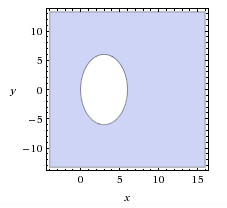
\includegraphics{ob1plot.png}
  \caption{Plot of $\mathcal{D}(f)$ in problem 1 (i).}
  \label{plot.p1}
\end{figure}

\begin{figure}[h]
  \centering
  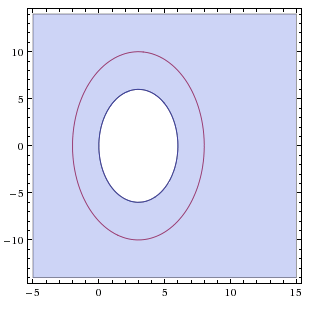
\includegraphics{ob1plot2.png}
  \caption{Plot of $C=0$ and $C=4$ in problem 1 (ii).}
  \label{plot.p2}
\end{figure}

\begin{figure}[h]
  \centering
  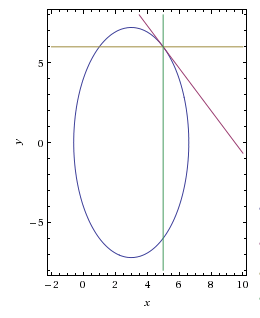
\includegraphics{ob1plot3.png}
  \caption{Plot of tangent line $\ell_{(5,6)}$ in problem 1 (iii).}
  \label{plot.p3}
\end{figure}

\end{document}
